\chapter{绪论}

\section{研究背景及意义}

区块链(Blockchain)是一种按照时间顺序将数据区块以链条的方式组成的特定数据结构,被视为分布式的共享账本和数据库。它能够使用户在无可信中介的情况下完成价值传输\cite{SurveyofEnterpriseBlockchains}。作为区块链2.0 的以太坊\footnotemark[1]\footnotetext[1]{\href{http://github.com/ethereum/wiki/wiki/White-Paper/}{以太坊白皮书}}重新将智能合约描述为部署于区块链网络中的合同条款代码。这意味着传统的合同条款可以进入实体计算机中,且在区块链网络去中心化、不可伪造、不可篡改的特性下严格执行。区块链推进了人与企业之间和线上与线下的全方面互联,其被称为新型生产关系。随着区块链的快速发展, 智能合约极大地丰富和扩展了区块链应用场景, 已经快速渗入到人们生活的方方面面。目前, 去中心化应用纷纷落地, 逐步从概念验证阶段转化为工程化实践阶段\footnotemark[2]\footnotetext[2]{\href{https://www.bilibili.com/video/BV1vK4y1A7pY?spm_id_from=333.337.search-card.all.click}{自动化框架 (BAF) 简介}}。

与此同时, 云原生(Cloud Native)是基于云的软件架构思想和软件开发实践的一组方法论, 因其弹性和分布式的优势成为当今流行的软件服务模式。云原生技术有利于各组织在公有云、私有云和混合云等新型动态环境中构建和运行可弹性扩展的应用。用户可以借助平台的全面自动化能力, 持续交付部署业务生产系统。

区块链即服务(Blockchain as a Service, 简称BaaS)则是基于云原生技术体系的一种构建、管理、托管和运维区块链网络及其应用的云服务平台\cite{onik2019performance}。BaaS支持将任何企业级区块链实施到云环境, 而无需任何IT专业知识。这大大降低了区块链技术的使用门槛, 是促使区块链技术更广泛、更深入地渗透到各个行业和企业的催化剂, 其市值预计从2018年的6.23亿美元猛增2023年的150亿美元\footnotemark[3]\footnotetext[3]{\href{https://www.reportbuyer.com/product/5486837/global-blockchain-as-a-service-market.html}{Global Blockchain-as-a-Service Market 2018-2022}}。市场发展迅速, 具有极大的商业价值。其中, 云厂商提供了大多数的BaaS平台\cite{KuernetesbasedFabricChaincodeManagementAndHihgAvailabilityTechnology}, 如表\ref{major_BaaS_platforms}所示, 其底层区块链支撑技术大多数选择IBM开源的跨企业级联盟链Hyperledger Fabric(简称HF), 这也是本文选择HF的原因。

{\footnotesize
\begin{longtable}[h]{m{100pt} m{50pt} m{50pt} m{50pt} m{50pt}}
    \caption[主要公有云的BaaS平台]{主要公有云的BaaS平台} \label{major_BaaS_platforms} \\
        \toprule  
        \textbf{BaaS平台}&\textbf{Ethereum}&\textbf{Quorum}&\textbf{Corda}&\textbf{HF}\\
        \hline
        
        AWS&Y&Y&Y&Y\\

        Azure&Y&Y&Y&Y\\

        IBM& & & &Y\\

        阿里云区块链服务&Y& & &Y\\

        腾讯云区块链服务TBaaS& & & &Y\\

        华为云区块链服务BCS& & & &Y\\
        \bottomrule
    \end{longtable}
}



% 挑战
BaaS基于云的自动化的能力屏蔽了底层区块链技术, 为上层去中心化应用提供了便捷地构建区块链网络等功能。然而, 软件工程中没有银弹, 当前区块链的发展依旧存在诸多挑战。

首先, 区块链基础商业化应用工具并不完善\footnotemark[1]\footnotetext[1]{\href{http://www.caict.ac.cn/kxyj/qwfb/ztbg/202107/P020210726503897354430.pdf}{区块链基础设施研究报告(2021年)}}。BaaS平台发展还处于初级阶段, 商业运行模式仍处在探索阶段。由于BaaS平台研发投入大, 目前市场上存在如AWS、IBM、阿里云区块链服务等多种BaaS平台解决方案, 这些BaaS平台计费高昂\footnotemark[2]\footnotetext[2]{\href{https://help.aliyun.com/document_detail/107710.html?spm=5176.14107623.commonbuy2container.1.59523b20xmyuNf}{阿里云区块链服务BaaS规格与定价}}并且与其他云服务捆绑销售。传统的企业业务或已存在稳定合作的云服务商, 使用不同云服务商的合作伙伴就需要跨云部署, 由于缺乏统一的顶层规划, 各云厂商的BaaS底层异构, 存在不可复用的跨解决方案的资源和工具, 这形成了多云的网络\cite{DBLP:conf/coins/GerritsKKFV21}、技术信息孤岛。同时, BaaS平台几乎都由互联网云服务巨头企业把控, 可用性限制通常会迫使企业为来自各种云提供商的基础设施即服务(Infrastructure as a Service, 简称IaaS)付费, 最终形成马太效应\cite{KuernetesbasedFabricChaincodeManagementAndHihgAvailabilityTechnology}。

其次, BaaS平台利用云能力对区块链基础设施赋能乏力。作为一种广泛部署的技术, 云计算是实施区块链技术的合适目标。然而, 区块链与云原生两种技术都相对不成熟, 两者的集成可能会在技术方面产生新的复杂性\cite{onik2019performance}。区块链服务比常规云服务更复杂, 问题仍然在于如何使区块链和云兼容\cite{gai2020blockchain}。目前, 行业缺少既定的标准或最佳实践范例, 各云厂商的BaaS解决方案基本都采取已有的开源解决方案, 业务同质化严重。具体地, 他们 仅提供一种基于开源区块链平台的自动部署管理方案, 未深入到区块链与云基础设施的底层。然而, 自动化脚本部署并不是有效的云化方式, 浪费了云原生技术的潜力。例如, 在数据存储备份及可扩展性方面, 随着交易数量的增加, 传统自动化部署方案无法利用云的弹性伸缩能力, 最终 出现存储膨胀问题。这限制了区块链的数据可扩展性, 所以需要结合云的能力寻找数据备份、升级及可扩展性的方法。区块链基础设施如何与云原生快速深度结合, 利用伸缩性、可移植性和高可用性的特性来提供“高质量”的区块链服务, 是当前仍然遗留的挑战。

最后, 区块链领域缺少促进去中心化应用价值交付的有效手段。去中心化应用价值交付很大程度上就意味着利用智能合约编写合同条款代码, 然而智能合约技术还处在初级阶段, 其相较于传统应用而言缺少既定的标准开发运维流程。具体地, 目前智能合约部署过程缺乏有效的自动化手段, 耗费大量的时间成本; 智能合约作为区块链的链上代码执行,安全问题产生会造成巨大的损失,合约代码在部署过程中缺乏有效的安全性验证,易导致代码漏洞; 智能合约运行过程, 缺乏有效的监控手段, 对智能合约运行过程中的负载等情况一无所知。对于大部分的去中心化应用开发组织来说,如何将传统成熟工具和新型智能合约应用联系起来, 仍是一个棘手的问题。

\begin{figure}[h] %figure环境,h默认参数是可以浮动,不是固定在当前位置。如果要不浮动,你就可以使用大写float宏包的H参数,固定图片在当前位置,禁止浮动。
    \centering %使图片居中显示
    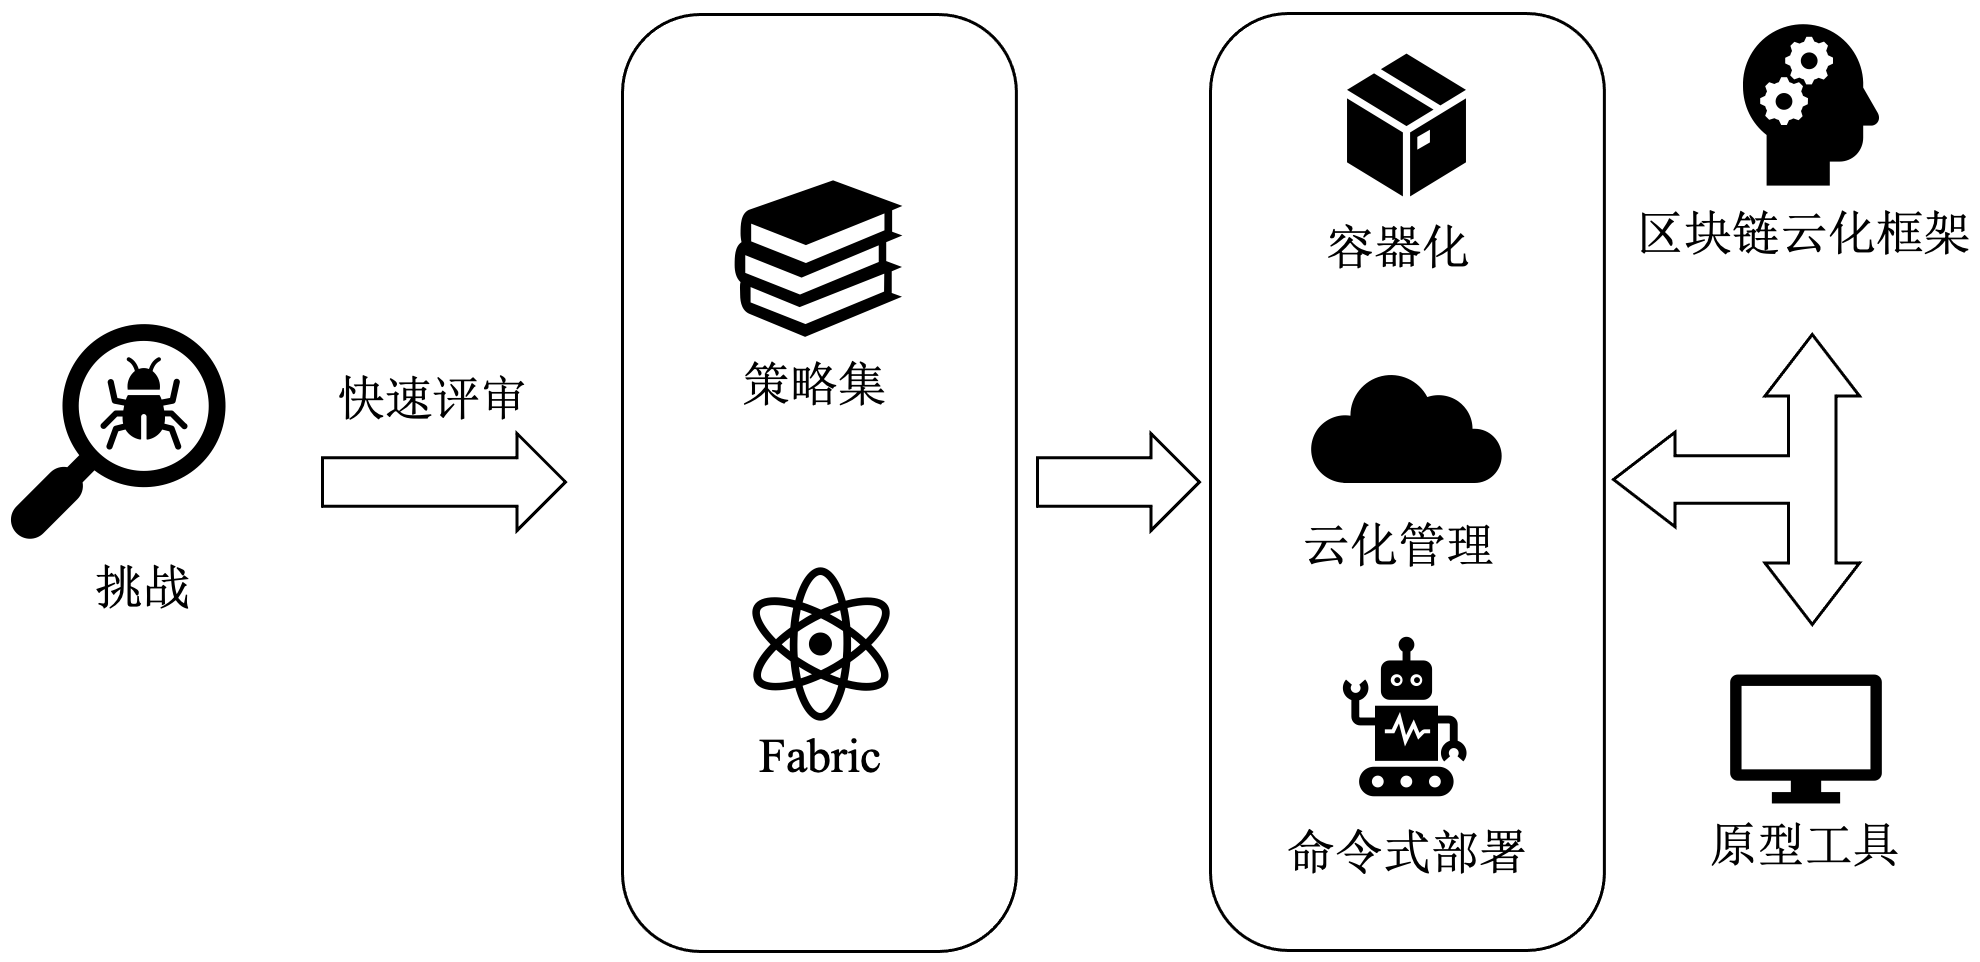
\includegraphics[width=1.0\textwidth]{FIGs/chapter1/process.png} %中括号中的参数是设置图片充满文档的大小,你也可以使用小数来缩小图片的尺寸。
    \caption{研究内容} %caption是用来给图片加上图题的
    \label{framework_tool} %这是添加标签,方便在文章中引用图片。
\end{figure}%figure环境


% 意义、愿景
针对上述问题, 本文选择面向联盟链场景的开源框架HF和Kubernetes提出了一种区块链云化框架, 包含了对下层区块链网络基础设施节点的云化以及智能合约的开发运维流程两个方面, 具体工作如图\ref{framework_tool}所示。在区块链网络节点云化方面, 本文对Kubernetes Operator进行了快速评审, 得到Kubernetes Operator云化赋能传统领域的策略集。然后, 本文结合HF网络的特性对策略集进行了筛选获得具体的节点云化方案。在智能合约的开发运维流程即价值交付方面, 本文首先对比了智能合约与微服务在设计原则上的相似性, 在此基础之上将智能合约进行微服务化改造, 包括智能合约与网络节点的解耦、运行环境、通信机制以及持续交付。智能合约经改造后能够有效利用传统成熟的工具支撑其开发运维工作。基于网络节点云化以及智能合约微服务化本文设计了面向Hyperledger Fabric的区块链云化框架。该框架对HF网络中的Ca、Orderer、Peer节点以及链码进行抽象适配并利用Kubernetes Operator进行完整生命周期管理, 利用智能合约微服务化流程将智能合约持续交付到云化节点。框架提升了HF网络的可移植性、可靠性、易用性、可扩展性以及安全性, 能够使HF网络获得类似云的自我管理, 使微服务的开发运维流程服务于智能合约领域。最终, 本文对框架及其原型工具从基本能力自证、成熟度衡量以及对比分析三个角度进行了测试与评估。在基本能力自证方面, 利用典型案例分析对原型工具进行了功能方面的可行性测试, 利用基于场景的SAAM架构方法对区块链基础设施的质量属性进行评估; 在成熟度衡量方面, 利用五层成熟度模型进行定性评估; 在对比分析方面, 与官方Cello对比进行定量评估。

\section{研究现状}

由于区块链智能合约的无法删除、修改、历史可追溯、去中心化、严格执行等特点, 越来越多的研究人员想挖掘区块链的潜能, 将区块链的能力应用到各种应用场景。McCorry等人\cite{mccorry2017smart}将区块链应用在电子投票领域, 实现了一个基于以太坊的去中心化互联网公开投票协议,公开投票网络是一种自助协议, 每个选民都控制着自己投票的隐私, 只有在所有人都参与的情况下才会被破坏, 这是第一个实现的不依赖任何可信的权威机构来计数和保护选民隐私的去中心化应用。Chang和Chen\cite{chang2020blockchain}在供应链领域进行了系统文献综述,表明传统的供应链活动涉及多个中介, 存在信任和性能问题,利用区块链的潜力可以更好地扰乱供应链运作性能、分布式治理和过程自动化。Zhang和Wen\cite{zhang2017iot}提出了一种物联网电子商务模型, 旨在重新设计传统电子商务模型中的许多元素,并借助区块链和智能合约技术在物联网上实现智能财产和付费数据的交易。Leka等人\cite{leka2019systematic}相信区块链技术将是下一个技术革命,同时表明区块链研究现阶段在物联网\cite{christidis2016blockchains}、医疗、教育、政府各个领域都有涉及。

目前, 去中心化应用逐步从概念验证阶段转变为工程化、商业化阶段。由于区块链的复杂性给网络的构建以及智能合约的部署、运维工作带来了严重的时间成本。在去中心化应用价值交付过程中, 存在对于区块链底层技术的易用性、部署效率、安全性等多方面的挑战。研究人员在区块链基础设施与云原生结合方面都开始了一定的探索, 除了利用区块链的特性提升云的能力外\cite{DBLP:journals/comcom/XieZZWH21}\cite{DBLP:conf/smartcloud/SunWY20}\cite{8457813}, 研究人员也都期望利用云的特性自动化地构建出易于弹性扩展、高可用的区块链平台。

% 学术
% 应用场景 BaaS平台往云上迁移
在学术研究方面, 研究人员探究如何有效利用云平台来部署区块链平台。Gerrits等人\cite{DBLP:conf/coins/GerritsKKFV21}在Kubernetes中部署了分布式账本Hyperledger Sawtooth\footnotemark[1]\footnotetext[1]{\href{https://github.com/hyperledger/sawtooth-core}{Hyperledger Sawtooth github地址}}, 并运行了一个用例。他们旨在探讨该用例在真实场景云部署中的可行性和可扩展性。Liang等人\cite{liangeduchain}针对教育领域数据共享和信息欺骗的问题构建了一个高可用的教育联盟区块链平台, 并实现了基于Kubernetes的HF部署, 实现了将链码纳入Kubernetes环境管理的目标。然而, Wan等人\cite{wan2018novel}指出当前主流的BaaS提供商通常采用API进行用户访问, 或者简单地将区块链应用迁移到云, 这会侵蚀不可信的机制并带来锁定风险。他们随后提出了一种新的服务范式来克服现有BaaS的局限性。基于HF的实施表明, 该范式可以缓解当前BaaS对区块链特征的侵蚀。在云原生底层基础设施方面研究人员关注与区块链结合的Kubernetes调度问题。才丽\cite{caili2018}在Kubernetes上面对PBFT和区块链的本身特性提出了静态调度和自适应算法。Shi等人\cite{9582270}为了解决云端实现PoS区块链工作负载的高效调度问题, 首次在云计算中设计和实现了基于Kubernetes的解决PoS区块链应用程序迁移成本的系统, 最大限度地减少了使用的Kubernetes工作节点数量以降低总体费用,而且还提出了一种高性能的Kubernetes调度方案HPKS以最大限度地利用工作节点进行在线Pod管理。在智能合约开发运维层面, Porru等人~\cite{porru2017blockchain}指出需要为软件工程师提供特定于区块链软件开发的工具与技术, 并将区块链实现的软件定义为面向区块链的软件(Blockchain-Oriented Softare,简称BOS), 将开发BOS的软件实践称为面向区块链的软件工程(Blockchain-Oriented Softare Engineering,简称BOSE)。Tonelli等人\cite{tonelli2018ethereum}在2018年就指出了微服务架构与智能合约结构之间的相似性, Hu等人\footnotemark[2]\footnotetext[2]{\href{http://pss-system.cnipa.gov.cn/sipopublicsearch/patentsearch/showViewList-jumpToView.shtml}{发明专利: 一种建立智能合约微服务化的方法}}提出一种建立智能合约的微服务化方法, 以期望将智能合约在Kubernetes上运行。

% 工业界
相比于学术研究, 工业领域的探索更加注重自动化实践。Hyperledger Cello\footnotemark[3]\footnotetext[3]{\href{https://github.com/hyperledger/cello}{Hyperledger Cello}}支持在多种底层基础设施上从头快速构建BaaS平台, 提供管理区块链网络的生命周期、自定义区块链网络配置等功能帮助人们以更高效的方式使用和管理区块链。Hyperledger Cello当前阶段重点关注在Docker安装, 对于Kubernetes的支持方面仍处在相对初级阶段, 配置项简单灵活性不足且老旧。Blockchain Automation Framework\footnotemark[1]\footnotetext[1]{\href{https://github.com/nikoturin/blockchain-automation-framework}{Blockchain Automation Framework}}提供了一个自动化框架, 利用Ansible\footnotemark[2]\footnotetext[2]{\href{https://github.com/ansible/ansible}{Ansible}}以及Helm\footnotemark[3]\footnotetext[3]{\href{https://github.com/helm/helm}{Helm}}快速地、一致地将生产就绪的分布式账本技术(Distributed ledger technology, 简称DLT)平台部署到云基础设施。虽然, Blockchain Automation Framework提供了一个自动化框架将区块链平台部署于Kubernetes, 但本质上还是描述为一个需要希望远程主机执行命令的方案,或者一组IT程序运行的命令集合。这大大提升了自动化程度, 但其远没有发挥Kubernetes的潜力。

% 总结
尽管学术界以及工业界目前已有一些关于区块链云化的探索与研究, 但研究重点多为如何自动化地将区块链平台向云上迁移, 并且区块链平台的性能往往由于许多影响因素而不稳定, 尤其是当它们部署在动态云环境中的时候。综上, 当前研究缺少构建支持云和区块链一体化的有效服务模型\cite{9582270}, 缺少在云中操作区块链的实证研究\cite{8790849}。

在云中操作应用程序就需要将应用程序部署进Kubernetes, 这个过程需要部署多种资源。虽然这些资源有标准定义的模板, 但目前手工创造定义这些资源会导致大量重复的代码并引入人为错误。Kubernetes Operator是将领域知识集成到Kubernetes API编排过程中的最新方法\cite{henning2021reproducible}。一部分研究利用Kubernetes Operator方法通过自动化的方式将云底层的效率、灵活性等多方面优势拓展到多种领域。Huang等人\cite{huang2021fly}提出了一个轻量级的遥感大数据处理云原生框架。该框架利用Kubernetes Operator融合Spark, 自动化配置Spark参数, 提升并行遥感图像融合算法的效率。Zhou等人\cite{zhou2021container}提出了Torque Operator对高性能负载(High Performance Computing, 简称HPC)进行管理, 利用容器化来提升HPC的效率及灵活性。除此之外, 在5G\cite{arouk20205g}\cite{wiranata2020automation}、医疗\cite{rouzbeh2020unified}等领域, Kubernetes Operator也发挥出其强大的自动化与编排能力, 利用云原生的可迁移性、可伸缩性、安全性等特性进行赋能, 但在区块链领域的Kubernetes Operator相关工作较少。


\section{本文贡献与主要研究工作}

% 侧重描述的,创新点,为什么被称为创新点,解决了其他工作没有解决的问题。工作解决了什么问题, 工作的创新点。

% 主要贡献
本文的研究目标是在云原生技术体系下, 更简单、更原生地管理HF。其核心价值体现在: (1)快速部署。 当前去中心化应用的价值交付过程有10\%到20\%的时间都花费在网络的启动和管理上, 尤其是还会出现更复杂的配置情况。(2)区块链云化框架并不是建立新的壁垒,而是避免云厂商的锁定。(3)提供云与区块链结合的实践范例, 包含区块链网络节点的云化方案以及智能合约微服务化的开发运维流程。(4)使网络根据业务可变。
如联盟中新的成员的加入、随数据膨胀而增加账本资源等, 这些改变通过规范化代码的角度而不是人工干预。

具体地, 本文的主要研究工作分为以下四个方面: 

1. 由于当前缺少云和区块链一体化有效服务模型, 所以针对区块链的基础设施即区块链网络节点。本文首先以Kubernetes Operator及其衍伸词汇为主题进行了快速评审, 快速评审的范围涵盖了计算机与软件工程领域的权威全文数据库。经过快速评审, 本文得到了Kubernetes Operator赋能传统领域提升软件质量属性的策略集。根据区块链云化设计原则并结合区块链网络的特性, 最终形成了区块链网络节点云化的具体实施方案。

2. 针对智能合约在开发运维过程中遇到的部署效率差、监控工具不完善等问题, 本文对比分析了微服务与智能合约在设计原则上的相似性。由于微服务与智能合约在设计原则上有很大的相似性, 这为本文智能合约微服务化改造奠定了良好基础。随后, 本文将智能合约在保证运行无误的前提下进行了微服务化改造。最后本文提出了智能合约微服务化开发运维流程, 其可以利用成熟的自动化工具对智能合约进行进行持续集成、持续部署与持续监控。

3. 基于上述区块链网络节点云化和智能合约微服务化开发运维方法, 本文设计实现了面向Hyperledger Fabric的区块链云化框架及其原型平台。框架自定义三种网络节点资源类型(Custom Resource Definition, 简称CRD)以及一种链码资源类型。这些CRD将区块链领域知识注入Kubernetes基础设施, 通过这种方式可以自动化配置网络, 消除人为错误, 提升云化框架的易用性。其次, Manager作为框架中枢处理单元对利用Helm对HF网络节点进行全生命周期管理, 并根据节点云化实施方案, 复用Kubernetes机制提升框架及HF网络节点的可移植性、可靠性、易用性、可扩展性以及安全性。
最后, HF网络作为框架的输出单元, 包含了维持HF网络节点运行的各种配置以及合理的运行状态。成功启动稳定的区块链网络后, 框架能够利用传统成熟的工具持续地将智能合约部署到云化的区块链网络上, 持续地向用户交付智能合约的价值。

4. 对原型平台进行了测试与评估。本文从以下三个维度对框架及其原型工具进行评估: 基础能力自证, 本文以典型案例的方式对原型工具进行了功能性测试, 利用SAAM架构评估方法验证网络节点的质量属性; 成熟度衡量, 本文结合五层成熟度模型对原型工具进行了定性评估; 对比分析, 本文与Hyperledger官方的BaaS工具Cello对比进行了定量评估。结果表明, 本文的原型工具在兼容区块链基本功能的前提下能够充分利用云的特性提升HF网络节点的可移植性、可靠性、易用性、可扩展性以及安全性, 利用智能合约微服务化的开发运维方法促进智能合约的价值交付过程。本文的原型工具可以基本满足五层成熟度模型的能力并且在网络部署时间和链码交付效率方面, 原型工具具有更优的表现。

\section{本文组织结构}

本文组织结构如下:

第一章~绪论。介绍了本文的研究背景及意义、国内外研究现状、工业界的主要探索以及本文主要的研究工作。

第二章~理论与技术支持。介绍了区块链尤其是HF的相关理论和概念; 同时介绍了云原生的基本概念发展历程, 并对云原生基础设施Kubernetes进行了详细介绍。

第三章~区块链网络节点云化方案。介绍了通过快速评审获得Kubernetes Operator赋能传统领域的策略集, 同时结合区块链云化设计原则以及区块链本身特性对策略集进行筛选得到具体云化实施方案。

第四章~智能合约微服务化开发运维方法。介绍了智能合约与微服务的设计原则, 同时基于这两者在设计原则上的相似性提出智能合约微服务化改造以及智能合约微服务化开发运维流程。

第五章~面向Hyperledger Fabric的区块链云化框架。介绍了本文提出的面向Hyperledger Fabric的区块链云化框架, 包含输入、处理以及输出单元; 介绍了原型工具的需求分析、设计与实现。

第六章~测试与评估。从基础能力自证、成熟度衡量以及对比分析三个维度对框架及原型工具进行测试与评估。

第七章~总结与展望。对全文进行总结; 阐述了区块链云化框架的局限性; 对未来工作进行了展望。


